\begin{scanpage}{0050}{33}
\begin{minipage}[t]{.45\linewidth}\vspace{0pt}\centering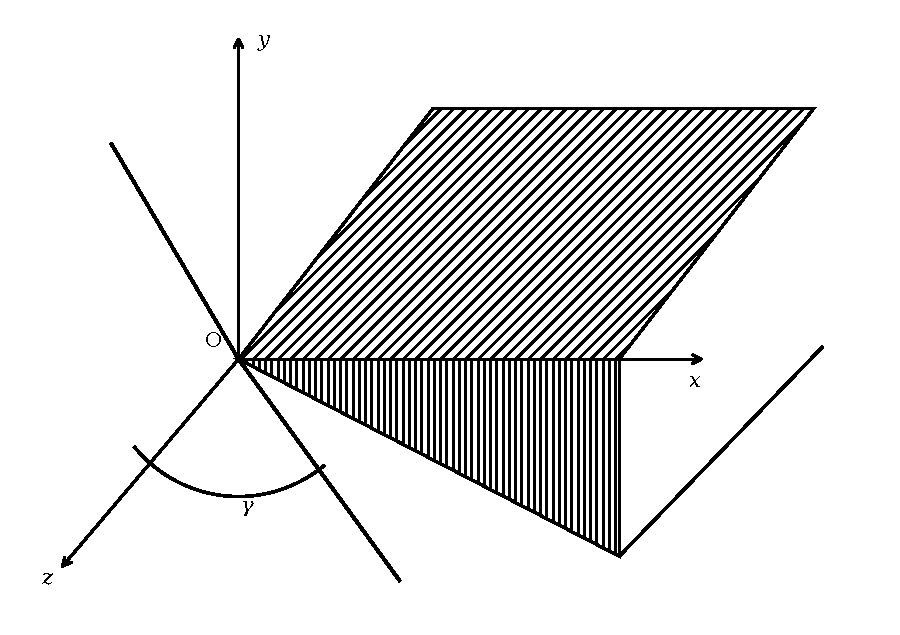
\includegraphics[width=.9\linewidth]{images/recreated/a-0050-fig14.pdf}\par Figure 14. Diffraction by a wedge with oblique incidence of a plane wave. $\gamma$ is the angle between the normal to the incident wave front and the $z$ axis.\end{minipage}\hfill\begin{minipage}[t]{.51\linewidth}\vspace{0pt}
\[\left.\begin{aligned}\mathbf E&=\mathbf E(x,y)e^{ikz\cos\gamma},\\\mathbf H&=\mathbf H(x,y)e^{ikz\cos\gamma}.\end{aligned}\right\}\tag{5.02}\]
Using Maxwell's equations
\[\operatorname{rot}\mathbf H=-ik\mathbf E,\quad\operatorname{rot}\mathbf E=ik\mathbf H,\tag{5.03}\]
one is able to obtain the following expressions for the radial and azimuthal components of the field:
\end{minipage}
\[\begin{aligned}E_r&=-\frac1{ik\sin^2\gamma}\left(\frac1r\frac{\partial H_z}{\partial\phi}+\cos\gamma\frac{\partial E_z}{\partial r}\right),\\H_r&=\frac1{ik\sin^2\gamma}\left(\frac1r\frac{\partial E_z}{\partial\phi}-\cos\gamma\frac{\partial H_z}{\partial r}\right),\\E_\phi&=\frac1{ik\sin^2\gamma}\left(\frac{\partial H_z}{\partial r}-\frac{\cos\gamma}r\frac{\partial E_z}{\partial\phi}\right),\\H_\phi&=-\frac1{ik\sin^2\gamma}\left(\frac{\partial E_z}{\partial r}+\frac{\cos\gamma}r\frac{\partial H_z}{\partial\phi}\right).\end{aligned}\tag{5.04}\]
The functions $E_z$ and $H_z$ in turn satisfy the wave equations
\[\Delta E_z+k_1^2E_z=0,\quad\Delta H_z+k_1^2H_z=0,\tag{5.05}\]
where
\[\Delta=\frac{\partial^2}{\partial x^2}+\frac{\partial^2}{\partial y^2}\quad\text{and }k_1=k\sin\gamma.\tag{5.06}\]
In \S\ 4 we found the fields (4.05) and (4.06) which satisfy the equations
\[\Delta E_z+k^2E_z=0,\quad\Delta H_z+k^2H_z=0\tag{5.07}\]
and which are created by the nonuniform part of the current excited on the wedge by the plane wave
\end{scanpage}
